\documentclass[1p]{elsarticle_modified}
%\bibliographystyle{elsarticle-num}

%\usepackage[colorlinks]{hyperref}
%\usepackage{abbrmath_seonhwa} %\Abb, \Ascr, \Acal ,\Abf, \Afrak
\usepackage{amsfonts}
\usepackage{amssymb}
\usepackage{amsmath}
\usepackage{amsthm}
\usepackage{scalefnt}
\usepackage{amsbsy}
\usepackage{kotex}
\usepackage{caption}
\usepackage{subfig}
\usepackage{color}
\usepackage{graphicx}
\usepackage{xcolor} %% white, black, red, green, blue, cyan, magenta, yellow
\usepackage{float}
\usepackage{setspace}
\usepackage{hyperref}

\usepackage{tikz}
\usetikzlibrary{arrows}

\usepackage{multirow}
\usepackage{array} % fixed length table
\usepackage{hhline}

%%%%%%%%%%%%%%%%%%%%%
\makeatletter
\renewcommand*\env@matrix[1][\arraystretch]{%
	\edef\arraystretch{#1}%
	\hskip -\arraycolsep
	\let\@ifnextchar\new@ifnextchar
	\array{*\c@MaxMatrixCols c}}
\makeatother %https://tex.stackexchange.com/questions/14071/how-can-i-increase-the-line-spacing-in-a-matrix
%%%%%%%%%%%%%%%

\usepackage[normalem]{ulem}

\newcommand{\msout}[1]{\ifmmode\text{\sout{\ensuremath{#1}}}\else\sout{#1}\fi}
%SOURCE: \msout is \stkout macro in https://tex.stackexchange.com/questions/20609/strikeout-in-math-mode

\newcommand{\cancel}[1]{
	\ifmmode
	{\color{red}\msout{#1}}
	\else
	{\color{red}\sout{#1}}
	\fi
}

\newcommand{\add}[1]{
	{\color{blue}\uwave{#1}}
}

\newcommand{\replace}[2]{
	\ifmmode
	{\color{red}\msout{#1}}{\color{blue}\uwave{#2}}
	\else
	{\color{red}\sout{#1}}{\color{blue}\uwave{#2}}
	\fi
}

\newcommand{\Sol}{\mathcal{S}} %segment
\newcommand{\D}{D} %diagram
\newcommand{\A}{\mathcal{A}} %arc


%%%%%%%%%%%%%%%%%%%%%%%%%%%%%5 test

\def\sl{\operatorname{\textup{SL}}(2,\Cbb)}
\def\psl{\operatorname{\textup{PSL}}(2,\Cbb)}
\def\quan{\mkern 1mu \triangleright \mkern 1mu}

\theoremstyle{definition}
\newtheorem{thm}{Theorem}[section]
\newtheorem{prop}[thm]{Proposition}
\newtheorem{lem}[thm]{Lemma}
\newtheorem{ques}[thm]{Question}
\newtheorem{cor}[thm]{Corollary}
\newtheorem{defn}[thm]{Definition}
\newtheorem{exam}[thm]{Example}
\newtheorem{rmk}[thm]{Remark}
\newtheorem{alg}[thm]{Algorithm}

\newcommand{\I}{\sqrt{-1}}
\begin{document}

%\begin{frontmatter}
%
%\title{Boundary parabolic representations of knots up to 8 crossings}
%
%%% Group authors per affiliation:
%\author{Yunhi Cho} 
%\address{Department of Mathematics, University of Seoul, Seoul, Korea}
%\ead{yhcho@uos.ac.kr}
%
%
%\author{Seonhwa Kim} %\fnref{s_kim}}
%\address{Center for Geometry and Physics, Institute for Basic Science, Pohang, 37673, Korea}
%\ead{ryeona17@ibs.re.kr}
%
%\author{Hyuk Kim}
%\address{Department of Mathematical Sciences, Seoul National University, Seoul 08826, Korea}
%\ead{hyukkim@snu.ac.kr}
%
%\author{Seokbeom Yoon}
%\address{Department of Mathematical Sciences, Seoul National University, Seoul, 08826,  Korea}
%\ead{sbyoon15@snu.ac.kr}
%
%\begin{abstract}
%We find all boundary parabolic representation of knots up to 8 crossings.
%
%\end{abstract}
%\begin{keyword}
%    \MSC[2010] 57M25 
%\end{keyword}
%
%\end{frontmatter}

%\linenumbers
%\tableofcontents
%
\newcommand\colored[1]{\textcolor{white}{\rule[-0.35ex]{0.8em}{1.4ex}}\kern-0.8em\color{red} #1}%
%\newcommand\colored[1]{\textcolor{white}{ #1}\kern-2.17ex	\textcolor{white}{ #1}\kern-1.81ex	\textcolor{white}{ #1}\kern-2.15ex\color{red}#1	}

{\Large $\underline{11a_{278}~(K11a_{278})}$}

\setlength{\tabcolsep}{10pt}
\renewcommand{\arraystretch}{1.6}
\vspace{1cm}\begin{tabular}{m{100pt}>{\centering\arraybackslash}m{274pt}}
\multirow{5}{120pt}{
	\centering
	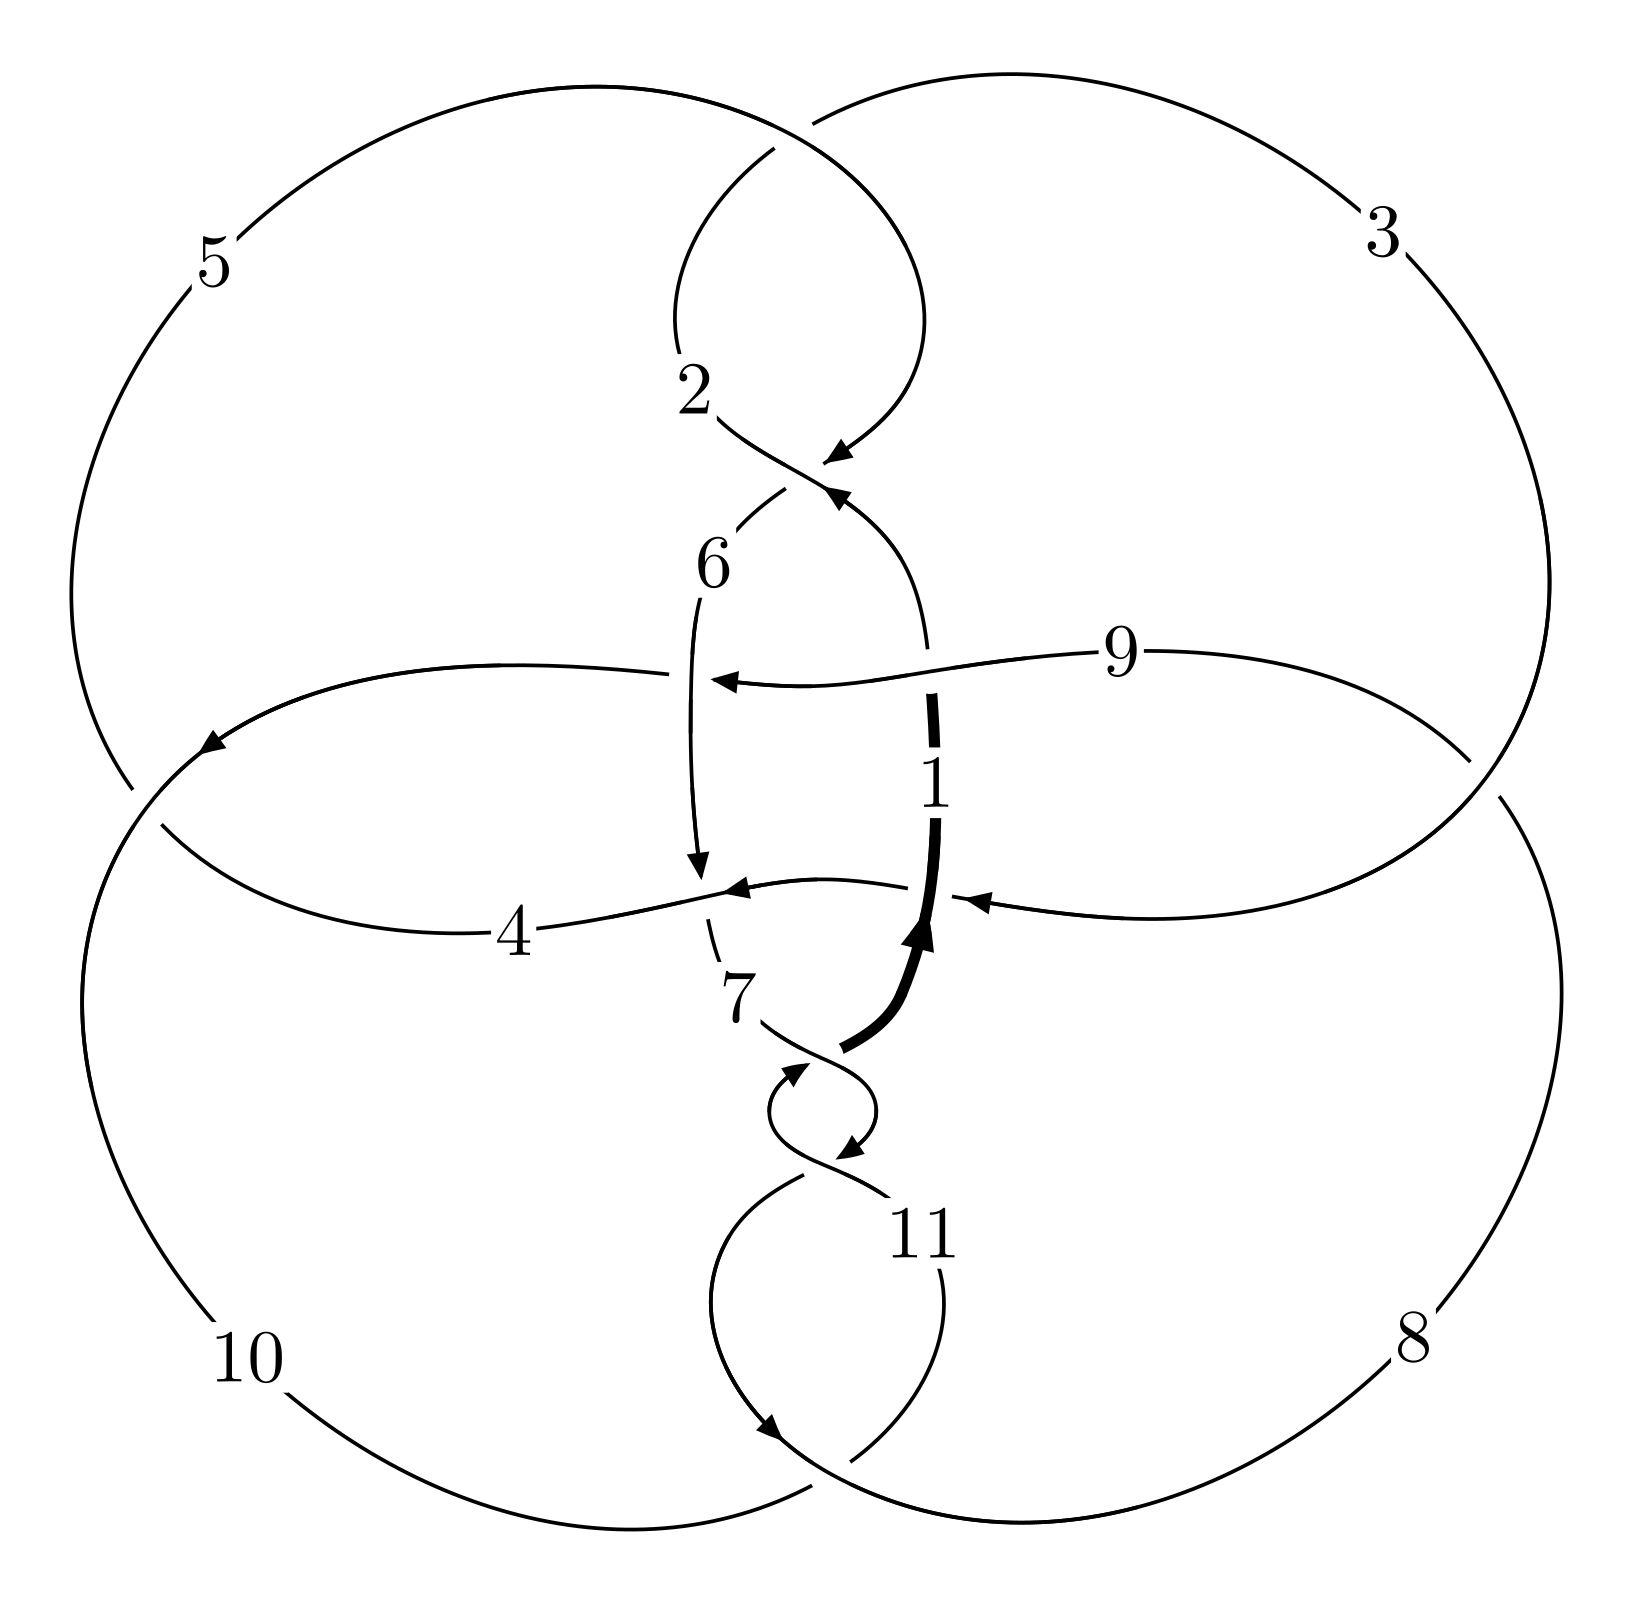
\includegraphics[width=112pt]{../../../GIT/diagram.site/Diagrams/png/527_11a_278.png}\\
\ \ \ A knot diagram\footnotemark}&
\allowdisplaybreaks
\textbf{Linearized knot diagam} \\
\cline{2-2}
 &
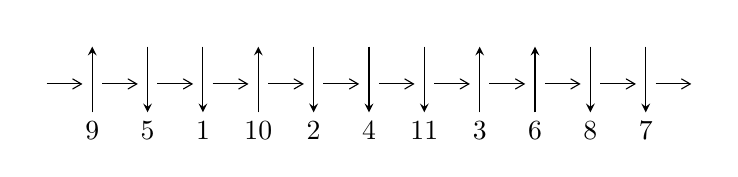
\begin{tikzpicture}[x=20pt, y=17pt]
	% nodes
	\node (C0) at (0, 0) {};
	\node (C1) at (1, 0) {};
	\node (C1U) at (1, +1) {};
	\node (C1D) at (1, -1) {9};

	\node (C2) at (2, 0) {};
	\node (C2U) at (2, +1) {};
	\node (C2D) at (2, -1) {5};

	\node (C3) at (3, 0) {};
	\node (C3U) at (3, +1) {};
	\node (C3D) at (3, -1) {1};

	\node (C4) at (4, 0) {};
	\node (C4U) at (4, +1) {};
	\node (C4D) at (4, -1) {10};

	\node (C5) at (5, 0) {};
	\node (C5U) at (5, +1) {};
	\node (C5D) at (5, -1) {2};

	\node (C6) at (6, 0) {};
	\node (C6U) at (6, +1) {};
	\node (C6D) at (6, -1) {4};

	\node (C7) at (7, 0) {};
	\node (C7U) at (7, +1) {};
	\node (C7D) at (7, -1) {11};

	\node (C8) at (8, 0) {};
	\node (C8U) at (8, +1) {};
	\node (C8D) at (8, -1) {3};

	\node (C9) at (9, 0) {};
	\node (C9U) at (9, +1) {};
	\node (C9D) at (9, -1) {6};

	\node (C10) at (10, 0) {};
	\node (C10U) at (10, +1) {};
	\node (C10D) at (10, -1) {8};

	\node (C11) at (11, 0) {};
	\node (C11U) at (11, +1) {};
	\node (C11D) at (11, -1) {7};
	\node (C12) at (12, 0) {};

	% arrows
	\draw[->,>={angle 60}]
	(C0) edge (C1) (C1) edge (C2) (C2) edge (C3) (C3) edge (C4) (C4) edge (C5) (C5) edge (C6) (C6) edge (C7) (C7) edge (C8) (C8) edge (C9) (C9) edge (C10) (C10) edge (C11) (C11) edge (C12) ;	\draw[->,>=stealth]
	(C1D) edge (C1U) (C2U) edge (C2D) (C3U) edge (C3D) (C4D) edge (C4U) (C5U) edge (C5D) (C6U) edge (C6D) (C7U) edge (C7D) (C8D) edge (C8U) (C9D) edge (C9U) (C10U) edge (C10D) (C11U) edge (C11D) ;
	\end{tikzpicture} \\
\hhline{~~} \\& 
\textbf{Solving Sequence} \\ \cline{2-2} 
 &
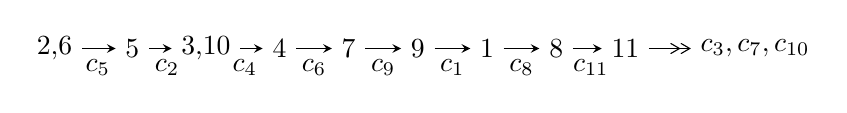
\begin{tikzpicture}[x=25pt, y=7pt]
	% node
	\node (A0) at (-1/8, 0) {2,6};
	\node (A1) at (1, 0) {5};
	\node (A2) at (33/16, 0) {3,10};
	\node (A3) at (25/8, 0) {4};
	\node (A4) at (33/8, 0) {7};
	\node (A5) at (41/8, 0) {9};
	\node (A6) at (49/8, 0) {1};
	\node (A7) at (57/8, 0) {8};
	\node (A8) at (65/8, 0) {11};
	\node (C1) at (1/2, -1) {$c_{5}$};
	\node (C2) at (3/2, -1) {$c_{2}$};
	\node (C3) at (21/8, -1) {$c_{4}$};
	\node (C4) at (29/8, -1) {$c_{6}$};
	\node (C5) at (37/8, -1) {$c_{9}$};
	\node (C6) at (45/8, -1) {$c_{1}$};
	\node (C7) at (53/8, -1) {$c_{8}$};
	\node (C8) at (61/8, -1) {$c_{11}$};
	\node (A9) at (10, 0) {$c_{3},c_{7},c_{10}$};

	% edge
	\draw[->,>=stealth]	
	(A0) edge (A1) (A1) edge (A2) (A2) edge (A3) (A3) edge (A4) (A4) edge (A5) (A5) edge (A6) (A6) edge (A7) (A7) edge (A8) ;
	\draw[->>,>={angle 60}]	
	(A8) edge (A9);
\end{tikzpicture} \\ 

\end{tabular} \\

\footnotetext{
The image of knot diagram is generated by the software ``\textbf{Draw programme}" developed by Andrew Bartholomew(\url{http://www.layer8.co.uk/maths/draw/index.htm\#Running-draw}), where we modified some parts for our purpose(\url{https://github.com/CATsTAILs/LinksPainter}).
}\phantom \\ \newline 
\centering \textbf{Ideals for irreducible components\footnotemark of $X_{\text{par}}$} 
 
\begin{align*}
I^u_{1}&=\langle 
1.19641\times10^{18} u^{40}-1.14397\times10^{19} u^{39}+\cdots+1.66044\times10^{18} b+1.81027\times10^{19},\\
\phantom{I^u_{1}}&\phantom{= \langle  }4.68165\times10^{19} u^{40}-5.02396\times10^{20} u^{39}+\cdots+3.98505\times10^{19} a-1.19786\times10^{21},\\
\phantom{I^u_{1}}&\phantom{= \langle  }u^{41}-11 u^{40}+\cdots-239 u+24\rangle \\
I^u_{2}&=\langle 
- u^{22} a-6 u^{21} a+\cdots- a-1,\;- u^{21} a-3 u^{22}+\cdots+a^2-13 u,\;u^{23}+7 u^{22}+\cdots+4 u+1\rangle \\
I^u_{3}&=\langle 
2 u^{15}+15 u^{14}+\cdots+b+8,\;-8 u^{16}-54 u^{15}+\cdots+5 a+43,\;u^{17}+8 u^{16}+\cdots+29 u+5\rangle \\
\\
\end{align*}
\raggedright * 3 irreducible components of $\dim_{\mathbb{C}}=0$, with total 104 representations.\\
\footnotetext{All coefficients of polynomials are rational numbers. But the coefficients are sometimes approximated in decimal forms when there is not enough margin.}
\newpage
\renewcommand{\arraystretch}{1}
\centering \section*{I. $I^u_{1}= \langle 1.20\times10^{18} u^{40}-1.14\times10^{19} u^{39}+\cdots+1.66\times10^{18} b+1.81\times10^{19},\;4.68\times10^{19} u^{40}-5.02\times10^{20} u^{39}+\cdots+3.99\times10^{19} a-1.20\times10^{21},\;u^{41}-11 u^{40}+\cdots-239 u+24 \rangle$}
\flushleft \textbf{(i) Arc colorings}\\
\begin{tabular}{m{7pt} m{180pt} m{7pt} m{180pt} }
\flushright $a_{2}=$&$\begin{pmatrix}0\\u\end{pmatrix}$ \\
\flushright $a_{6}=$&$\begin{pmatrix}1\\0\end{pmatrix}$ \\
\flushright $a_{5}=$&$\begin{pmatrix}1\\- u^2\end{pmatrix}$ \\
\flushright $a_{3}=$&$\begin{pmatrix}- u\\u^3+u\end{pmatrix}$ \\
\flushright $a_{10}=$&$\begin{pmatrix}-1.17480 u^{40}+12.6070 u^{39}+\cdots-319.545 u+30.0588\\-0.720540 u^{40}+6.88956 u^{39}+\cdots+67.6080 u-10.9023\end{pmatrix}$ \\
\flushright $a_{4}=$&$\begin{pmatrix}1.14574 u^{40}-11.8183 u^{39}+\cdots-20.0365 u+6.80811\\0.738778 u^{40}-6.60293 u^{39}+\cdots-93.3051 u+9.76711\end{pmatrix}$ \\
\flushright $a_{7}=$&$\begin{pmatrix}0.633150 u^{40}-5.52375 u^{39}+\cdots-208.982 u+22.2813\\-0.938766 u^{40}+10.6746 u^{39}+\cdots-322.499 u+32.6119\end{pmatrix}$ \\
\flushright $a_{9}=$&$\begin{pmatrix}-0.454264 u^{40}+5.71745 u^{39}+\cdots-387.153 u+40.9611\\-0.720540 u^{40}+6.88956 u^{39}+\cdots+67.6080 u-10.9023\end{pmatrix}$ \\
\flushright $a_{1}=$&$\begin{pmatrix}-1.28278 u^{40}+13.4475 u^{39}+\cdots-94.7279 u+10.9155\\0.663004 u^{40}-8.31978 u^{39}+\cdots+296.668 u-30.7866\end{pmatrix}$ \\
\flushright $a_{8}=$&$\begin{pmatrix}0.277139 u^{40}-1.62154 u^{39}+\cdots-383.007 u+40.2112\\-0.534336 u^{40}+6.09950 u^{39}+\cdots-87.8238 u+6.80221\end{pmatrix}$ \\
\flushright $a_{11}=$&$\begin{pmatrix}-2.29615 u^{40}+24.6191 u^{39}+\cdots-309.565 u+27.7328\\-0.339712 u^{40}+2.80144 u^{39}+\cdots+173.961 u-19.8874\end{pmatrix}$\\ \flushright $a_{11}=$&$\begin{pmatrix}-2.29615 u^{40}+24.6191 u^{39}+\cdots-309.565 u+27.7328\\-0.339712 u^{40}+2.80144 u^{39}+\cdots+173.961 u-19.8874\end{pmatrix}$\\&\end{tabular}
\flushleft \textbf{(ii) Obstruction class $= -1$}\\~\\
\flushleft \textbf{(iii) Cusp Shapes $= \frac{1664141169681345798}{1660437713445795359} u^{40}-\frac{20019045792937126226}{1660437713445795359} u^{39}+\cdots+\frac{734545644265820275638}{1660437713445795359} u-\frac{59737924674909497694}{1660437713445795359}$}\\~\\
\newpage\renewcommand{\arraystretch}{1}
\flushleft \textbf{(iv) u-Polynomials at the component}\newline \\
\begin{tabular}{m{50pt}|m{274pt}}
Crossings & \hspace{64pt}u-Polynomials at each crossing \\
\hline $$\begin{aligned}c_{1},c_{9}\end{aligned}$$&$\begin{aligned}
&u^{41}-12 u^{39}+\cdots-2 u+1
\end{aligned}$\\
\hline $$\begin{aligned}c_{2},c_{5}\end{aligned}$$&$\begin{aligned}
&u^{41}-11 u^{40}+\cdots-239 u+24
\end{aligned}$\\
\hline $$\begin{aligned}c_{3},c_{6}\end{aligned}$$&$\begin{aligned}
&u^{41}- u^{40}+\cdots+6 u+1
\end{aligned}$\\
\hline $$\begin{aligned}c_{4},c_{8}\end{aligned}$$&$\begin{aligned}
&u^{41}-3 u^{39}+\cdots+39 u+19
\end{aligned}$\\
\hline $$\begin{aligned}c_{7},c_{10},c_{11}\end{aligned}$$&$\begin{aligned}
&u^{41}-8 u^{40}+\cdots+9 u-2
\end{aligned}$\\
\hline
\end{tabular}\\~\\
\newpage\renewcommand{\arraystretch}{1}
\flushleft \textbf{(v) Riley Polynomials at the component}\newline \\
\begin{tabular}{m{50pt}|m{274pt}}
Crossings & \hspace{64pt}Riley Polynomials at each crossing \\
\hline $$\begin{aligned}c_{1},c_{9}\end{aligned}$$&$\begin{aligned}
&y^{41}-24 y^{40}+\cdots+96 y-1
\end{aligned}$\\
\hline $$\begin{aligned}c_{2},c_{5}\end{aligned}$$&$\begin{aligned}
&y^{41}+23 y^{40}+\cdots-10223 y-576
\end{aligned}$\\
\hline $$\begin{aligned}c_{3},c_{6}\end{aligned}$$&$\begin{aligned}
&y^{41}+27 y^{40}+\cdots-82 y-1
\end{aligned}$\\
\hline $$\begin{aligned}c_{4},c_{8}\end{aligned}$$&$\begin{aligned}
&y^{41}-6 y^{40}+\cdots+4637 y-361
\end{aligned}$\\
\hline $$\begin{aligned}c_{7},c_{10},c_{11}\end{aligned}$$&$\begin{aligned}
&y^{41}+40 y^{40}+\cdots-87 y-4
\end{aligned}$\\
\hline
\end{tabular}\\~\\
\newpage\flushleft \textbf{(vi) Complex Volumes and Cusp Shapes}
$$\begin{array}{c|c|c}  
\text{Solutions to }I^u_{1}& \I (\text{vol} + \sqrt{-1}CS) & \text{Cusp shape}\\
 \hline 
\begin{aligned}
u &= -0.029022 + 1.006330 I \\
a &= \phantom{-}1.62224 + 0.62151 I \\
b &= \phantom{-}1.118340 - 0.475258 I\end{aligned}
 & \phantom{-}3.33397 + 0.06687 I & \phantom{-}6.02301 + 0.24252 I \\ \hline\begin{aligned}
u &= -0.029022 - 1.006330 I \\
a &= \phantom{-}1.62224 - 0.62151 I \\
b &= \phantom{-}1.118340 + 0.475258 I\end{aligned}
 & \phantom{-}3.33397 - 0.06687 I & \phantom{-}6.02301 - 0.24252 I \\ \hline\begin{aligned}
u &= \phantom{-}0.212627 + 0.952062 I \\
a &= \phantom{-}1.81242 - 0.15435 I \\
b &= \phantom{-}0.78122 - 1.20521 I\end{aligned}
 & \phantom{-}1.10287 - 3.44596 I & -5.05254 - 2.71451 I \\ \hline\begin{aligned}
u &= \phantom{-}0.212627 - 0.952062 I \\
a &= \phantom{-}1.81242 + 0.15435 I \\
b &= \phantom{-}0.78122 + 1.20521 I\end{aligned}
 & \phantom{-}1.10287 + 3.44596 I & -5.05254 + 2.71451 I \\ \hline\begin{aligned}
u &= \phantom{-}1.052800 + 0.131390 I \\
a &= \phantom{-}0.017775 - 0.158160 I \\
b &= -0.971790 - 0.691117 I\end{aligned}
 & \phantom{-}0.26528 + 7.29842 I & -3.00000 - 7.62825 I \\ \hline\begin{aligned}
u &= \phantom{-}1.052800 - 0.131390 I \\
a &= \phantom{-}0.017775 + 0.158160 I \\
b &= -0.971790 + 0.691117 I\end{aligned}
 & \phantom{-}0.26528 - 7.29842 I & -3.00000 + 7.62825 I \\ \hline\begin{aligned}
u &= -0.125412 + 1.084050 I \\
a &= -1.83248 - 0.48717 I \\
b &= -1.204160 + 0.550939 I\end{aligned}
 & \phantom{-}8.77240 + 0.69151 I & \phantom{-}5.83897 + 1.00152 I \\ \hline\begin{aligned}
u &= -0.125412 - 1.084050 I \\
a &= -1.83248 + 0.48717 I \\
b &= -1.204160 - 0.550939 I\end{aligned}
 & \phantom{-}8.77240 - 0.69151 I & \phantom{-}5.83897 - 1.00152 I \\ \hline\begin{aligned}
u &= -1.12668\phantom{ +0.000000I} \\
a &= -0.245548\phantom{ +0.000000I} \\
b &= -0.130087\phantom{ +0.000000I}\end{aligned}
 & -2.19078\phantom{ +0.000000I} & -19.8800\phantom{ +0.000000I} \\ \hline\begin{aligned}
u &= \phantom{-}0.821173 + 0.119690 I \\
a &= -0.297539 + 0.031863 I \\
b &= \phantom{-}0.933904 + 0.677894 I\end{aligned}
 & \phantom{-}0.99974 + 2.62993 I & -0.91222 - 3.18628 I\\
 \hline 
 \end{array}$$\newpage$$\begin{array}{c|c|c}  
\text{Solutions to }I^u_{1}& \I (\text{vol} + \sqrt{-1}CS) & \text{Cusp shape}\\
 \hline 
\begin{aligned}
u &= \phantom{-}0.821173 - 0.119690 I \\
a &= -0.297539 - 0.031863 I \\
b &= \phantom{-}0.933904 - 0.677894 I\end{aligned}
 & \phantom{-}0.99974 - 2.62993 I & -0.91222 + 3.18628 I \\ \hline\begin{aligned}
u &= \phantom{-}1.182590 + 0.075770 I \\
a &= \phantom{-}0.116810 + 0.162777 I \\
b &= \phantom{-}0.978144 + 0.696826 I\end{aligned}
 & \phantom{-}6.46948 + 11.04650 I & \phantom{-0.000000 } 0. - 7.47384 I \\ \hline\begin{aligned}
u &= \phantom{-}1.182590 - 0.075770 I \\
a &= \phantom{-}0.116810 - 0.162777 I \\
b &= \phantom{-}0.978144 - 0.696826 I\end{aligned}
 & \phantom{-}6.46948 - 11.04650 I & \phantom{-0.000000 -}0. + 7.47384 I \\ \hline\begin{aligned}
u &= -0.388375 + 1.153130 I \\
a &= \phantom{-}0.886517 + 0.002500 I \\
b &= \phantom{-}0.509537 - 0.312406 I\end{aligned}
 & \phantom{-}5.35338 + 3.81903 I & \phantom{-0.000000 } 0 \\ \hline\begin{aligned}
u &= -0.388375 - 1.153130 I \\
a &= \phantom{-}0.886517 - 0.002500 I \\
b &= \phantom{-}0.509537 + 0.312406 I\end{aligned}
 & \phantom{-}5.35338 - 3.81903 I & \phantom{-0.000000 } 0 \\ \hline\begin{aligned}
u &= \phantom{-}0.717608 + 0.311811 I \\
a &= -0.110757 - 0.623250 I \\
b &= -1.032150 + 0.566413 I\end{aligned}
 & \phantom{-}7.82283 - 0.16471 I & \phantom{-}3.38955 + 1.65431 I \\ \hline\begin{aligned}
u &= \phantom{-}0.717608 - 0.311811 I \\
a &= -0.110757 + 0.623250 I \\
b &= -1.032150 - 0.566413 I\end{aligned}
 & \phantom{-}7.82283 + 0.16471 I & \phantom{-}3.38955 - 1.65431 I \\ \hline\begin{aligned}
u &= \phantom{-}0.495810 + 1.155840 I \\
a &= \phantom{-}0.816045 + 0.781921 I \\
b &= \phantom{-}1.125660 - 0.059155 I\end{aligned}
 & \phantom{-}4.52174 - 1.46436 I & \phantom{-0.000000 } 0 \\ \hline\begin{aligned}
u &= \phantom{-}0.495810 - 1.155840 I \\
a &= \phantom{-}0.816045 - 0.781921 I \\
b &= \phantom{-}1.125660 + 0.059155 I\end{aligned}
 & \phantom{-}4.52174 + 1.46436 I & \phantom{-0.000000 } 0 \\ \hline\begin{aligned}
u &= -1.215000 + 0.331445 I \\
a &= \phantom{-}0.383654 - 0.112321 I \\
b &= \phantom{-}0.206819 - 0.088073 I\end{aligned}
 & \phantom{-}1.95983 + 1.37588 I & \phantom{-0.000000 } 0\\
 \hline 
 \end{array}$$\newpage$$\begin{array}{c|c|c}  
\text{Solutions to }I^u_{1}& \I (\text{vol} + \sqrt{-1}CS) & \text{Cusp shape}\\
 \hline 
\begin{aligned}
u &= -1.215000 - 0.331445 I \\
a &= \phantom{-}0.383654 + 0.112321 I \\
b &= \phantom{-}0.206819 + 0.088073 I\end{aligned}
 & \phantom{-}1.95983 - 1.37588 I & \phantom{-0.000000 } 0 \\ \hline\begin{aligned}
u &= \phantom{-}0.038850 + 0.715738 I \\
a &= -1.55374 - 1.28578 I \\
b &= -1.154670 + 0.349145 I\end{aligned}
 & \phantom{-}7.32305 + 0.14265 I & \phantom{-}5.03936 + 0.27284 I \\ \hline\begin{aligned}
u &= \phantom{-}0.038850 - 0.715738 I \\
a &= -1.55374 + 1.28578 I \\
b &= -1.154670 - 0.349145 I\end{aligned}
 & \phantom{-}7.32305 - 0.14265 I & \phantom{-}5.03936 - 0.27284 I \\ \hline\begin{aligned}
u &= -0.185808 + 0.685986 I \\
a &= -1.118850 + 0.444113 I \\
b &= -0.249566 + 0.572464 I\end{aligned}
 & -0.087291 + 1.322900 I & -3.26673 - 3.24423 I \\ \hline\begin{aligned}
u &= -0.185808 - 0.685986 I \\
a &= -1.118850 - 0.444113 I \\
b &= -0.249566 - 0.572464 I\end{aligned}
 & -0.087291 - 1.322900 I & -3.26673 + 3.24423 I \\ \hline\begin{aligned}
u &= \phantom{-}0.347665 + 1.264830 I \\
a &= -1.77476 - 0.18019 I \\
b &= -1.31566 + 0.98619 I\end{aligned}
 & \phantom{-}12.33800 - 3.83464 I & \phantom{-0.000000 } 0 \\ \hline\begin{aligned}
u &= \phantom{-}0.347665 - 1.264830 I \\
a &= -1.77476 + 0.18019 I \\
b &= -1.31566 - 0.98619 I\end{aligned}
 & \phantom{-}12.33800 + 3.83464 I & \phantom{-0.000000 } 0 \\ \hline\begin{aligned}
u &= \phantom{-}0.490892 + 1.239610 I \\
a &= \phantom{-}1.70373 + 0.26449 I \\
b &= \phantom{-}1.40330 - 0.98654 I\end{aligned}
 & \phantom{-}4.41136 - 7.49164 I & \phantom{-0.000000 } 0 \\ \hline\begin{aligned}
u &= \phantom{-}0.490892 - 1.239610 I \\
a &= \phantom{-}1.70373 - 0.26449 I \\
b &= \phantom{-}1.40330 + 0.98654 I\end{aligned}
 & \phantom{-}4.41136 + 7.49164 I & \phantom{-0.000000 } 0 \\ \hline\begin{aligned}
u &= \phantom{-}0.684336 + 1.194050 I \\
a &= -0.636884 - 0.796428 I \\
b &= -1.128510 - 0.133079 I\end{aligned}
 & \phantom{-}10.00540 - 5.34593 I & \phantom{-0.000000 } 0\\
 \hline 
 \end{array}$$\newpage$$\begin{array}{c|c|c}  
\text{Solutions to }I^u_{1}& \I (\text{vol} + \sqrt{-1}CS) & \text{Cusp shape}\\
 \hline 
\begin{aligned}
u &= \phantom{-}0.684336 - 1.194050 I \\
a &= -0.636884 + 0.796428 I \\
b &= -1.128510 + 0.133079 I\end{aligned}
 & \phantom{-}10.00540 + 5.34593 I & \phantom{-0.000000 } 0 \\ \hline\begin{aligned}
u &= \phantom{-}0.325776 + 1.364770 I \\
a &= -0.829707 - 0.563437 I \\
b &= -0.920142 + 0.089185 I\end{aligned}
 & \phantom{-}5.42164 + 2.35534 I & \phantom{-0.000000 } 0 \\ \hline\begin{aligned}
u &= \phantom{-}0.325776 - 1.364770 I \\
a &= -0.829707 + 0.563437 I \\
b &= -0.920142 - 0.089185 I\end{aligned}
 & \phantom{-}5.42164 - 2.35534 I & \phantom{-0.000000 } 0 \\ \hline\begin{aligned}
u &= \phantom{-}0.558892 + 1.297930 I \\
a &= -1.62402 - 0.22838 I \\
b &= -1.40055 + 0.94692 I\end{aligned}
 & \phantom{-}3.92238 - 13.02370 I & \phantom{-0.000000 } 0 \\ \hline\begin{aligned}
u &= \phantom{-}0.558892 - 1.297930 I \\
a &= -1.62402 + 0.22838 I \\
b &= -1.40055 - 0.94692 I\end{aligned}
 & \phantom{-}3.92238 + 13.02370 I & \phantom{-0.000000 } 0 \\ \hline\begin{aligned}
u &= \phantom{-}0.58068 + 1.35810 I \\
a &= \phantom{-}1.60234 + 0.17682 I \\
b &= \phantom{-}1.38863 - 0.93704 I\end{aligned}
 & \phantom{-}10.5240 - 17.2112 I & \phantom{-0.000000 } 0 \\ \hline\begin{aligned}
u &= \phantom{-}0.58068 - 1.35810 I \\
a &= \phantom{-}1.60234 - 0.17682 I \\
b &= \phantom{-}1.38863 + 0.93704 I\end{aligned}
 & \phantom{-}10.5240 + 17.2112 I & \phantom{-0.000000 } 0 \\ \hline\begin{aligned}
u &= \phantom{-}0.113639 + 0.464794 I \\
a &= -1.43312 + 0.66702 I \\
b &= \phantom{-}0.144535 + 0.741778 I\end{aligned}
 & -0.006980 + 1.308310 I & \phantom{-}1.77615 - 2.91870 I \\ \hline\begin{aligned}
u &= \phantom{-}0.113639 - 0.464794 I \\
a &= -1.43312 - 0.66702 I \\
b &= \phantom{-}0.144535 - 0.741778 I\end{aligned}
 & -0.006980 - 1.308310 I & \phantom{-}1.77615 + 2.91870 I \\ \hline\begin{aligned}
u &= \phantom{-}0.38362 + 1.54611 I \\
a &= \phantom{-}0.727259 + 0.513748 I \\
b &= \phantom{-}0.852167 - 0.006427 I\end{aligned}
 & \phantom{-}11.91810 + 4.98494 I & \phantom{-0.000000 } 0\\
 \hline 
 \end{array}$$\newpage$$\begin{array}{c|c|c}  
\text{Solutions to }I^u_{1}& \I (\text{vol} + \sqrt{-1}CS) & \text{Cusp shape}\\
 \hline 
\begin{aligned}
u &= \phantom{-}0.38362 - 1.54611 I \\
a &= \phantom{-}0.727259 - 0.513748 I \\
b &= \phantom{-}0.852167 + 0.006427 I\end{aligned}
 & \phantom{-}11.91810 - 4.98494 I & \phantom{-0.000000 } 0\\
 \hline 
 \end{array}$$\newpage\newpage\renewcommand{\arraystretch}{1}
\centering \section*{II. $I^u_{2}= \langle - u^{22} a-6 u^{21} a+\cdots- a-1,\;- u^{21} a-3 u^{22}+\cdots+a^2-13 u,\;u^{23}+7 u^{22}+\cdots+4 u+1 \rangle$}
\flushleft \textbf{(i) Arc colorings}\\
\begin{tabular}{m{7pt} m{180pt} m{7pt} m{180pt} }
\flushright $a_{2}=$&$\begin{pmatrix}0\\u\end{pmatrix}$ \\
\flushright $a_{6}=$&$\begin{pmatrix}1\\0\end{pmatrix}$ \\
\flushright $a_{5}=$&$\begin{pmatrix}1\\- u^2\end{pmatrix}$ \\
\flushright $a_{3}=$&$\begin{pmatrix}- u\\u^3+u\end{pmatrix}$ \\
\flushright $a_{10}=$&$\begin{pmatrix}a\\u^{22} a+6 u^{21} a+\cdots+a+1\end{pmatrix}$ \\
\flushright $a_{4}=$&$\begin{pmatrix}- u^{21}-8 u^{20}+\cdots- a-3\\- u^{22} a-6 u^{21} a+\cdots- a-1\end{pmatrix}$ \\
\flushright $a_{7}=$&$\begin{pmatrix}- u^{21}-6 u^{20}+\cdots- a+3\\u^{22} a+6 u^{21} a+\cdots+a-1\end{pmatrix}$ \\
\flushright $a_{9}=$&$\begin{pmatrix}- u^{22} a-6 u^{21} a+\cdots-4 u-1\\u^{22} a+6 u^{21} a+\cdots+a+1\end{pmatrix}$ \\
\flushright $a_{1}=$&$\begin{pmatrix}- u^{21} a- u^{21}+\cdots+a+4\\-1\end{pmatrix}$ \\
\flushright $a_{8}=$&$\begin{pmatrix}u^{21}+6 u^{20}+\cdots+a-1\\- u^{22} a-6 u^{21} a+\cdots- a+1\end{pmatrix}$ \\
\flushright $a_{11}=$&$\begin{pmatrix}- u^{21}-6 u^{20}+\cdots+a+2\\u^{22} a+6 u^{21} a+\cdots+a-1\end{pmatrix}$\\ \flushright $a_{11}=$&$\begin{pmatrix}- u^{21}-6 u^{20}+\cdots+a+2\\u^{22} a+6 u^{21} a+\cdots+a-1\end{pmatrix}$\\&\end{tabular}
\flushleft \textbf{(ii) Obstruction class $= -1$}\\~\\
\flushleft \textbf{(iii) Cusp Shapes $= -4 u^{22}-20 u^{21}-72 u^{20}-172 u^{19}-320 u^{18}-444 u^{17}-436 u^{16}-196 u^{15}+308 u^{14}+932 u^{13}+1500 u^{12}+1784 u^{11}+1704 u^{10}+1348 u^9+844 u^8+436 u^7+148 u^6+16 u^5-20 u^4-28 u^3-4 u^2-8 u-6$}\\~\\
\newpage\renewcommand{\arraystretch}{1}
\flushleft \textbf{(iv) u-Polynomials at the component}\newline \\
\begin{tabular}{m{50pt}|m{274pt}}
Crossings & \hspace{64pt}u-Polynomials at each crossing \\
\hline $$\begin{aligned}c_{1},c_{9}\end{aligned}$$&$\begin{aligned}
&u^{46}- u^{45}+\cdots+8 u^2+1
\end{aligned}$\\
\hline $$\begin{aligned}c_{2},c_{5}\end{aligned}$$&$\begin{aligned}
&(u^{23}+7 u^{22}+\cdots+4 u+1)^{2}
\end{aligned}$\\
\hline $$\begin{aligned}c_{3},c_{6}\end{aligned}$$&$\begin{aligned}
&u^{46}-7 u^{45}+\cdots-188 u+37
\end{aligned}$\\
\hline $$\begin{aligned}c_{4},c_{8}\end{aligned}$$&$\begin{aligned}
&u^{46}+u^{45}+\cdots+36 u+11
\end{aligned}$\\
\hline $$\begin{aligned}c_{7},c_{10},c_{11}\end{aligned}$$&$\begin{aligned}
&(u^{23}+5 u^{22}+\cdots+6 u^2-1)^{2}
\end{aligned}$\\
\hline
\end{tabular}\\~\\
\newpage\renewcommand{\arraystretch}{1}
\flushleft \textbf{(v) Riley Polynomials at the component}\newline \\
\begin{tabular}{m{50pt}|m{274pt}}
Crossings & \hspace{64pt}Riley Polynomials at each crossing \\
\hline $$\begin{aligned}c_{1},c_{9}\end{aligned}$$&$\begin{aligned}
&y^{46}+7 y^{45}+\cdots+16 y+1
\end{aligned}$\\
\hline $$\begin{aligned}c_{2},c_{5}\end{aligned}$$&$\begin{aligned}
&(y^{23}+15 y^{22}+\cdots-12 y-1)^{2}
\end{aligned}$\\
\hline $$\begin{aligned}c_{3},c_{6}\end{aligned}$$&$\begin{aligned}
&y^{46}-5 y^{45}+\cdots+23412 y+1369
\end{aligned}$\\
\hline $$\begin{aligned}c_{4},c_{8}\end{aligned}$$&$\begin{aligned}
&y^{46}-13 y^{45}+\cdots+4820 y+121
\end{aligned}$\\
\hline $$\begin{aligned}c_{7},c_{10},c_{11}\end{aligned}$$&$\begin{aligned}
&(y^{23}+23 y^{22}+\cdots+12 y-1)^{2}
\end{aligned}$\\
\hline
\end{tabular}\\~\\
\newpage\flushleft \textbf{(vi) Complex Volumes and Cusp Shapes}
$$\begin{array}{c|c|c}  
\text{Solutions to }I^u_{2}& \I (\text{vol} + \sqrt{-1}CS) & \text{Cusp shape}\\
 \hline 
\begin{aligned}
u &= \phantom{-}0.233567 + 1.031350 I \\
a &= \phantom{-}0.34801 + 1.50362 I \\
b &= \phantom{-}0.60058 + 2.13953 I\end{aligned}
 & \phantom{-}7.62895 - 7.86344 I & \phantom{-}3.61806 + 10.44591 I \\ \hline\begin{aligned}
u &= \phantom{-}0.233567 + 1.031350 I \\
a &= -2.69560 + 0.51605 I \\
b &= -0.596857 + 0.409017 I\end{aligned}
 & \phantom{-}7.62895 - 7.86344 I & \phantom{-}3.61806 + 10.44591 I \\ \hline\begin{aligned}
u &= \phantom{-}0.233567 - 1.031350 I \\
a &= \phantom{-}0.34801 - 1.50362 I \\
b &= \phantom{-}0.60058 - 2.13953 I\end{aligned}
 & \phantom{-}7.62895 + 7.86344 I & \phantom{-}3.61806 - 10.44591 I \\ \hline\begin{aligned}
u &= \phantom{-}0.233567 - 1.031350 I \\
a &= -2.69560 - 0.51605 I \\
b &= -0.596857 - 0.409017 I\end{aligned}
 & \phantom{-}7.62895 + 7.86344 I & \phantom{-}3.61806 - 10.44591 I \\ \hline\begin{aligned}
u &= \phantom{-}0.186753 + 0.913593 I \\
a &= \phantom{-}0.54495 - 1.43828 I \\
b &= \phantom{-}0.02137 - 2.03091 I\end{aligned}
 & \phantom{-}0.48240 - 3.68961 I & -4.31455 + 10.86650 I \\ \hline\begin{aligned}
u &= \phantom{-}0.186753 + 0.913593 I \\
a &= \phantom{-}2.57289 - 0.13037 I \\
b &= \phantom{-}0.443646 - 0.589013 I\end{aligned}
 & \phantom{-}0.48240 - 3.68961 I & -4.31455 + 10.86650 I \\ \hline\begin{aligned}
u &= \phantom{-}0.186753 - 0.913593 I \\
a &= \phantom{-}0.54495 + 1.43828 I \\
b &= \phantom{-}0.02137 + 2.03091 I\end{aligned}
 & \phantom{-}0.48240 + 3.68961 I & -4.31455 - 10.86650 I \\ \hline\begin{aligned}
u &= \phantom{-}0.186753 - 0.913593 I \\
a &= \phantom{-}2.57289 + 0.13037 I \\
b &= \phantom{-}0.443646 + 0.589013 I\end{aligned}
 & \phantom{-}0.48240 + 3.68961 I & -4.31455 - 10.86650 I \\ \hline\begin{aligned}
u &= -1.07372\phantom{ +0.000000I} \\
a &= -0.257664 + 0.016236 I \\
b &= -0.133412 + 0.236476 I\end{aligned}
 & -2.18491\phantom{ +0.000000I} & -16.7310\phantom{ +0.000000I} \\ \hline\begin{aligned}
u &= -1.07372\phantom{ +0.000000I} \\
a &= -0.257664 - 0.016236 I \\
b &= -0.133412 - 0.236476 I\end{aligned}
 & -2.18491\phantom{ +0.000000I} & -16.7310\phantom{ +0.000000I}\\
 \hline 
 \end{array}$$\newpage$$\begin{array}{c|c|c}  
\text{Solutions to }I^u_{2}& \I (\text{vol} + \sqrt{-1}CS) & \text{Cusp shape}\\
 \hline 
\begin{aligned}
u &= -1.126300 + 0.206470 I \\
a &= \phantom{-}0.499507 - 0.147399 I \\
b &= \phantom{-}0.427226 + 0.266230 I\end{aligned}
 & \phantom{-}1.93766 + 1.32101 I & -4.99704 - 4.34736 I \\ \hline\begin{aligned}
u &= -1.126300 + 0.206470 I \\
a &= \phantom{-}0.321072 - 0.184827 I \\
b &= -0.003992 - 0.480793 I\end{aligned}
 & \phantom{-}1.93766 + 1.32101 I & -4.99704 - 4.34736 I \\ \hline\begin{aligned}
u &= -1.126300 - 0.206470 I \\
a &= \phantom{-}0.499507 + 0.147399 I \\
b &= \phantom{-}0.427226 - 0.266230 I\end{aligned}
 & \phantom{-}1.93766 - 1.32101 I & -4.99704 + 4.34736 I \\ \hline\begin{aligned}
u &= -1.126300 - 0.206470 I \\
a &= \phantom{-}0.321072 + 0.184827 I \\
b &= -0.003992 + 0.480793 I\end{aligned}
 & \phantom{-}1.93766 - 1.32101 I & -4.99704 + 4.34736 I \\ \hline\begin{aligned}
u &= -0.616588 + 1.034050 I \\
a &= \phantom{-}1.49907 - 0.31690 I \\
b &= \phantom{-}1.218300 + 0.349141 I\end{aligned}
 & \phantom{-}4.52825 + 4.72419 I & -0.87243 - 5.66443 I \\ \hline\begin{aligned}
u &= -0.616588 + 1.034050 I \\
a &= -0.246425 + 0.316671 I \\
b &= -0.515604 - 0.701003 I\end{aligned}
 & \phantom{-}4.52825 + 4.72419 I & -0.87243 - 5.66443 I \\ \hline\begin{aligned}
u &= -0.616588 - 1.034050 I \\
a &= \phantom{-}1.49907 + 0.31690 I \\
b &= \phantom{-}1.218300 - 0.349141 I\end{aligned}
 & \phantom{-}4.52825 - 4.72419 I & -0.87243 + 5.66443 I \\ \hline\begin{aligned}
u &= -0.616588 - 1.034050 I \\
a &= -0.246425 - 0.316671 I \\
b &= -0.515604 + 0.701003 I\end{aligned}
 & \phantom{-}4.52825 - 4.72419 I & -0.87243 + 5.66443 I \\ \hline\begin{aligned}
u &= -0.356806 + 1.198900 I \\
a &= -0.908631 + 0.827801 I \\
b &= -0.674442 - 0.472287 I\end{aligned}
 & \phantom{-}4.04810 + 4.55921 I & \phantom{-}5.41713 - 6.09867 I \\ \hline\begin{aligned}
u &= -0.356806 + 1.198900 I \\
a &= \phantom{-}1.68320 + 0.12017 I \\
b &= \phantom{-}1.47512 + 0.74465 I\end{aligned}
 & \phantom{-}4.04810 + 4.55921 I & \phantom{-}5.41713 - 6.09867 I\\
 \hline 
 \end{array}$$\newpage$$\begin{array}{c|c|c}  
\text{Solutions to }I^u_{2}& \I (\text{vol} + \sqrt{-1}CS) & \text{Cusp shape}\\
 \hline 
\begin{aligned}
u &= -0.356806 - 1.198900 I \\
a &= -0.908631 - 0.827801 I \\
b &= -0.674442 + 0.472287 I\end{aligned}
 & \phantom{-}4.04810 - 4.55921 I & \phantom{-}5.41713 + 6.09867 I \\ \hline\begin{aligned}
u &= -0.356806 - 1.198900 I \\
a &= \phantom{-}1.68320 - 0.12017 I \\
b &= \phantom{-}1.47512 - 0.74465 I\end{aligned}
 & \phantom{-}4.04810 - 4.55921 I & \phantom{-}5.41713 + 6.09867 I \\ \hline\begin{aligned}
u &= \phantom{-}0.089537 + 0.682903 I \\
a &= -1.058990 - 0.734558 I \\
b &= \phantom{-}0.199185 + 0.887413 I\end{aligned}
 & -0.19963 + 1.69919 I & -7.29306 - 0.59779 I \\ \hline\begin{aligned}
u &= \phantom{-}0.089537 + 0.682903 I \\
a &= -2.31010 + 1.12368 I \\
b &= -0.994995 + 1.004440 I\end{aligned}
 & -0.19963 + 1.69919 I & -7.29306 - 0.59779 I \\ \hline\begin{aligned}
u &= \phantom{-}0.089537 - 0.682903 I \\
a &= -1.058990 + 0.734558 I \\
b &= \phantom{-}0.199185 - 0.887413 I\end{aligned}
 & -0.19963 - 1.69919 I & -7.29306 + 0.59779 I \\ \hline\begin{aligned}
u &= \phantom{-}0.089537 - 0.682903 I \\
a &= -2.31010 - 1.12368 I \\
b &= -0.994995 - 1.004440 I\end{aligned}
 & -0.19963 - 1.69919 I & -7.29306 + 0.59779 I \\ \hline\begin{aligned}
u &= -0.184645 + 1.327800 I \\
a &= -1.58659 - 0.65447 I \\
b &= -1.47802 - 1.24587 I\end{aligned}
 & \phantom{-}11.44280 + 6.01561 I & \phantom{-}9.34351 - 5.45649 I \\ \hline\begin{aligned}
u &= -0.184645 + 1.327800 I \\
a &= \phantom{-}1.53384 - 0.96668 I \\
b &= \phantom{-}0.765206 + 0.253347 I\end{aligned}
 & \phantom{-}11.44280 + 6.01561 I & \phantom{-}9.34351 - 5.45649 I \\ \hline\begin{aligned}
u &= -0.184645 - 1.327800 I \\
a &= -1.58659 + 0.65447 I \\
b &= -1.47802 + 1.24587 I\end{aligned}
 & \phantom{-}11.44280 - 6.01561 I & \phantom{-}9.34351 + 5.45649 I \\ \hline\begin{aligned}
u &= -0.184645 - 1.327800 I \\
a &= \phantom{-}1.53384 + 0.96668 I \\
b &= \phantom{-}0.765206 - 0.253347 I\end{aligned}
 & \phantom{-}11.44280 - 6.01561 I & \phantom{-}9.34351 + 5.45649 I\\
 \hline 
 \end{array}$$\newpage$$\begin{array}{c|c|c}  
\text{Solutions to }I^u_{2}& \I (\text{vol} + \sqrt{-1}CS) & \text{Cusp shape}\\
 \hline 
\begin{aligned}
u &= -0.54822 + 1.33148 I \\
a &= \phantom{-}0.914945 - 0.015844 I \\
b &= \phantom{-}0.843719 + 0.814001 I\end{aligned}
 & \phantom{-}1.92714 + 5.73570 I & -6.54258 - 11.45569 I \\ \hline\begin{aligned}
u &= -0.54822 + 1.33148 I \\
a &= -1.365520 + 0.207271 I \\
b &= -1.065870 - 0.549777 I\end{aligned}
 & \phantom{-}1.92714 + 5.73570 I & -6.54258 - 11.45569 I \\ \hline\begin{aligned}
u &= -0.54822 - 1.33148 I \\
a &= \phantom{-}0.914945 + 0.015844 I \\
b &= \phantom{-}0.843719 - 0.814001 I\end{aligned}
 & \phantom{-}1.92714 - 5.73570 I & -6.54258 + 11.45569 I \\ \hline\begin{aligned}
u &= -0.54822 - 1.33148 I \\
a &= -1.365520 - 0.207271 I \\
b &= -1.065870 + 0.549777 I\end{aligned}
 & \phantom{-}1.92714 - 5.73570 I & -6.54258 + 11.45569 I \\ \hline\begin{aligned}
u &= -0.388479 + 0.400318 I \\
a &= -1.155830 - 0.149061 I \\
b &= \phantom{-}0.438402 + 0.600768 I\end{aligned}
 & -0.02603 + 1.77955 I & -5.09313 - 4.79070 I \\ \hline\begin{aligned}
u &= -0.388479 + 0.400318 I \\
a &= -1.14506 + 1.66093 I \\
b &= -0.919497 + 0.346909 I\end{aligned}
 & -0.02603 + 1.77955 I & -5.09313 - 4.79070 I \\ \hline\begin{aligned}
u &= -0.388479 - 0.400318 I \\
a &= -1.155830 + 0.149061 I \\
b &= \phantom{-}0.438402 - 0.600768 I\end{aligned}
 & -0.02603 - 1.77955 I & -5.09313 + 4.79070 I \\ \hline\begin{aligned}
u &= -0.388479 - 0.400318 I \\
a &= -1.14506 - 1.66093 I \\
b &= -0.919497 - 0.346909 I\end{aligned}
 & -0.02603 - 1.77955 I & -5.09313 + 4.79070 I \\ \hline\begin{aligned}
u &= \phantom{-}0.300297 + 0.396341 I \\
a &= -0.36424 + 1.38690 I \\
b &= -0.583913 - 0.986914 I\end{aligned}
 & \phantom{-}5.91614 + 5.40360 I & -0.73363 - 1.75125 I \\ \hline\begin{aligned}
u &= \phantom{-}0.300297 + 0.396341 I \\
a &= \phantom{-}3.16595 - 0.53729 I \\
b &= \phantom{-}0.874871 - 0.799916 I\end{aligned}
 & \phantom{-}5.91614 + 5.40360 I & -0.73363 - 1.75125 I\\
 \hline 
 \end{array}$$\newpage$$\begin{array}{c|c|c}  
\text{Solutions to }I^u_{2}& \I (\text{vol} + \sqrt{-1}CS) & \text{Cusp shape}\\
 \hline 
\begin{aligned}
u &= \phantom{-}0.300297 - 0.396341 I \\
a &= -0.36424 - 1.38690 I \\
b &= -0.583913 + 0.986914 I\end{aligned}
 & \phantom{-}5.91614 - 5.40360 I & -0.73363 + 1.75125 I \\ \hline\begin{aligned}
u &= \phantom{-}0.300297 - 0.396341 I \\
a &= \phantom{-}3.16595 + 0.53729 I \\
b &= \phantom{-}0.874871 + 0.799916 I\end{aligned}
 & \phantom{-}5.91614 - 5.40360 I & -0.73363 + 1.75125 I \\ \hline\begin{aligned}
u &= -0.55226 + 1.43648 I \\
a &= -0.920559 - 0.249915 I \\
b &= -0.878187 - 0.988227 I\end{aligned}
 & \phantom{-}6.99739 + 7.32012 I & \phantom{-}2.83321 - 9.36955 I \\ \hline\begin{aligned}
u &= -0.55226 + 1.43648 I \\
a &= \phantom{-}1.43177 - 0.29444 I \\
b &= \phantom{-}1.037170 + 0.468605 I\end{aligned}
 & \phantom{-}6.99739 + 7.32012 I & \phantom{-}2.83321 - 9.36955 I \\ \hline\begin{aligned}
u &= -0.55226 - 1.43648 I \\
a &= -0.920559 + 0.249915 I \\
b &= -0.878187 + 0.988227 I\end{aligned}
 & \phantom{-}6.99739 - 7.32012 I & \phantom{-}2.83321 + 9.36955 I \\ \hline\begin{aligned}
u &= -0.55226 - 1.43648 I \\
a &= \phantom{-}1.43177 + 0.29444 I \\
b &= \phantom{-}1.037170 - 0.468605 I\end{aligned}
 & \phantom{-}6.99739 - 7.32012 I & \phantom{-}2.83321 + 9.36955 I\\
 \hline 
 \end{array}$$\newpage\newpage\renewcommand{\arraystretch}{1}
\centering \section*{III. $I^u_{3}= \langle 2 u^{15}+15 u^{14}+\cdots+b+8,\;-8 u^{16}-54 u^{15}+\cdots+5 a+43,\;u^{17}+8 u^{16}+\cdots+29 u+5 \rangle$}
\flushleft \textbf{(i) Arc colorings}\\
\begin{tabular}{m{7pt} m{180pt} m{7pt} m{180pt} }
\flushright $a_{2}=$&$\begin{pmatrix}0\\u\end{pmatrix}$ \\
\flushright $a_{6}=$&$\begin{pmatrix}1\\0\end{pmatrix}$ \\
\flushright $a_{5}=$&$\begin{pmatrix}1\\- u^2\end{pmatrix}$ \\
\flushright $a_{3}=$&$\begin{pmatrix}- u\\u^3+u\end{pmatrix}$ \\
\flushright $a_{10}=$&$\begin{pmatrix}\frac{8}{5} u^{16}+\frac{54}{5} u^{15}+\cdots-44 u-\frac{43}{5}\\-2 u^{15}-15 u^{14}+\cdots-47 u-8\end{pmatrix}$ \\
\flushright $a_{4}=$&$\begin{pmatrix}\frac{1}{5} u^{16}+\frac{8}{5} u^{15}+\cdots+19 u+\frac{24}{5}\\- u^2- u-1\end{pmatrix}$ \\
\flushright $a_{7}=$&$\begin{pmatrix}-\frac{1}{5} u^{16}-\frac{8}{5} u^{15}+\cdots-17 u-\frac{14}{5}\\u^4+2 u^3+3 u^2+2 u+1\end{pmatrix}$ \\
\flushright $a_{9}=$&$\begin{pmatrix}\frac{8}{5} u^{16}+\frac{64}{5} u^{15}+\cdots+3 u-\frac{3}{5}\\-2 u^{15}-15 u^{14}+\cdots-47 u-8\end{pmatrix}$ \\
\flushright $a_{1}=$&$\begin{pmatrix}\frac{4}{5} u^{16}+\frac{32}{5} u^{15}+\cdots+8 u-\frac{4}{5}\\- u^{15}-7 u^{14}+\cdots-23 u-4\end{pmatrix}$ \\
\flushright $a_{8}=$&$\begin{pmatrix}\frac{8}{5} u^{16}+\frac{59}{5} u^{15}+\cdots-28 u-\frac{28}{5}\\-2 u^{15}-15 u^{14}+\cdots-45 u-8\end{pmatrix}$ \\
\flushright $a_{11}=$&$\begin{pmatrix}\frac{2}{5} u^{16}+\frac{11}{5} u^{15}+\cdots-39 u-\frac{42}{5}\\- u^{15}-7 u^{14}+\cdots-16 u-2\end{pmatrix}$\\ \flushright $a_{11}=$&$\begin{pmatrix}\frac{2}{5} u^{16}+\frac{11}{5} u^{15}+\cdots-39 u-\frac{42}{5}\\- u^{15}-7 u^{14}+\cdots-16 u-2\end{pmatrix}$\\&\end{tabular}
\flushleft \textbf{(ii) Obstruction class $= 1$}\\~\\
\flushleft \textbf{(iii) Cusp Shapes $= -8 u^{16}-73 u^{15}-345 u^{14}-1129 u^{13}-2811 u^{12}-5603 u^{11}-9220 u^{10}-12735 u^9-14949 u^8-15016 u^7-12923 u^6-9534 u^5-5946 u^4-3070 u^3-1267 u^2-373 u-64$}\\~\\
\newpage\renewcommand{\arraystretch}{1}
\flushleft \textbf{(iv) u-Polynomials at the component}\newline \\
\begin{tabular}{m{50pt}|m{274pt}}
Crossings & \hspace{64pt}u-Polynomials at each crossing \\
\hline $$\begin{aligned}c_{1},c_{9}\end{aligned}$$&$\begin{aligned}
&u^{17}+3 u^{15}+\cdots- u-1
\end{aligned}$\\
\hline $$\begin{aligned}c_{2}\end{aligned}$$&$\begin{aligned}
&u^{17}-8 u^{16}+\cdots+29 u-5
\end{aligned}$\\
\hline $$\begin{aligned}c_{3},c_{6}\end{aligned}$$&$\begin{aligned}
&u^{17}+u^{16}+\cdots+u+1
\end{aligned}$\\
\hline $$\begin{aligned}c_{4},c_{8}\end{aligned}$$&$\begin{aligned}
&u^{17}-4 u^{15}+\cdots-2 u^2+1
\end{aligned}$\\
\hline $$\begin{aligned}c_{5}\end{aligned}$$&$\begin{aligned}
&u^{17}+8 u^{16}+\cdots+29 u+5
\end{aligned}$\\
\hline $$\begin{aligned}c_{7}\end{aligned}$$&$\begin{aligned}
&u^{17}-5 u^{16}+\cdots+6 u-1
\end{aligned}$\\
\hline $$\begin{aligned}c_{10},c_{11}\end{aligned}$$&$\begin{aligned}
&u^{17}+5 u^{16}+\cdots+6 u+1
\end{aligned}$\\
\hline
\end{tabular}\\~\\
\newpage\renewcommand{\arraystretch}{1}
\flushleft \textbf{(v) Riley Polynomials at the component}\newline \\
\begin{tabular}{m{50pt}|m{274pt}}
Crossings & \hspace{64pt}Riley Polynomials at each crossing \\
\hline $$\begin{aligned}c_{1},c_{9}\end{aligned}$$&$\begin{aligned}
&y^{17}+6 y^{16}+\cdots+7 y-1
\end{aligned}$\\
\hline $$\begin{aligned}c_{2},c_{5}\end{aligned}$$&$\begin{aligned}
&y^{17}+8 y^{16}+\cdots-159 y-25
\end{aligned}$\\
\hline $$\begin{aligned}c_{3},c_{6}\end{aligned}$$&$\begin{aligned}
&y^{17}-7 y^{16}+\cdots+y-1
\end{aligned}$\\
\hline $$\begin{aligned}c_{4},c_{8}\end{aligned}$$&$\begin{aligned}
&y^{17}-8 y^{16}+\cdots+4 y-1
\end{aligned}$\\
\hline $$\begin{aligned}c_{7},c_{10},c_{11}\end{aligned}$$&$\begin{aligned}
&y^{17}+17 y^{16}+\cdots-8 y-1
\end{aligned}$\\
\hline
\end{tabular}\\~\\
\newpage\flushleft \textbf{(vi) Complex Volumes and Cusp Shapes}
$$\begin{array}{c|c|c}  
\text{Solutions to }I^u_{3}& \I (\text{vol} + \sqrt{-1}CS) & \text{Cusp shape}\\
 \hline 
\begin{aligned}
u &= -0.212883 + 0.989804 I \\
a &= -1.78717 - 0.40799 I \\
b &= -0.65506 - 1.31329 I\end{aligned}
 & \phantom{-}1.43397 + 3.72395 I & \phantom{-}9.02521 - 8.71756 I \\ \hline\begin{aligned}
u &= -0.212883 - 0.989804 I \\
a &= -1.78717 + 0.40799 I \\
b &= -0.65506 + 1.31329 I\end{aligned}
 & \phantom{-}1.43397 - 3.72395 I & \phantom{-}9.02521 + 8.71756 I \\ \hline\begin{aligned}
u &= \phantom{-}0.187789 + 0.804462 I \\
a &= -1.56094 - 1.01561 I \\
b &= -0.263040 - 1.039610 I\end{aligned}
 & \phantom{-}7.01302 - 6.58132 I & \phantom{-}2.73271 + 4.66890 I \\ \hline\begin{aligned}
u &= \phantom{-}0.187789 - 0.804462 I \\
a &= -1.56094 + 1.01561 I \\
b &= -0.263040 + 1.039610 I\end{aligned}
 & \phantom{-}7.01302 + 6.58132 I & \phantom{-}2.73271 - 4.66890 I \\ \hline\begin{aligned}
u &= -0.049862 + 0.811132 I \\
a &= \phantom{-}1.77966 + 0.76282 I \\
b &= \phantom{-}0.299763 + 1.223360 I\end{aligned}
 & \phantom{-}0.38103 - 2.23066 I & \phantom{-}3.27072 + 6.66488 I \\ \hline\begin{aligned}
u &= -0.049862 - 0.811132 I \\
a &= \phantom{-}1.77966 - 0.76282 I \\
b &= \phantom{-}0.299763 - 1.223360 I\end{aligned}
 & \phantom{-}0.38103 + 2.23066 I & \phantom{-}3.27072 - 6.66488 I \\ \hline\begin{aligned}
u &= -1.26194\phantom{ +0.000000I} \\
a &= -0.0920978\phantom{ +0.000000I} \\
b &= -0.443696\phantom{ +0.000000I}\end{aligned}
 & -1.98855\phantom{ +0.000000I} & \phantom{-}20.3120\phantom{ +0.000000I} \\ \hline\begin{aligned}
u &= -0.623402 + 0.351291 I \\
a &= \phantom{-}0.635918 + 0.086672 I \\
b &= -0.381807 + 0.805862 I\end{aligned}
 & -0.81423 - 1.18978 I & -7.16259 + 1.41463 I \\ \hline\begin{aligned}
u &= -0.623402 - 0.351291 I \\
a &= \phantom{-}0.635918 - 0.086672 I \\
b &= -0.381807 - 0.805862 I\end{aligned}
 & -0.81423 + 1.18978 I & -7.16259 - 1.41463 I \\ \hline\begin{aligned}
u &= -0.159792 + 1.337940 I \\
a &= \phantom{-}1.264290 + 0.275164 I \\
b &= \phantom{-}0.691210 + 0.860233 I\end{aligned}
 & \phantom{-}9.78949 + 6.03317 I & \phantom{-}3.31072 - 5.48564 I\\
 \hline 
 \end{array}$$\newpage$$\begin{array}{c|c|c}  
\text{Solutions to }I^u_{3}& \I (\text{vol} + \sqrt{-1}CS) & \text{Cusp shape}\\
 \hline 
\begin{aligned}
u &= -0.159792 - 1.337940 I \\
a &= \phantom{-}1.264290 - 0.275164 I \\
b &= \phantom{-}0.691210 - 0.860233 I\end{aligned}
 & \phantom{-}9.78949 - 6.03317 I & \phantom{-}3.31072 + 5.48564 I \\ \hline\begin{aligned}
u &= -0.459989 + 1.288470 I \\
a &= -1.256360 + 0.121374 I \\
b &= -0.988881 - 0.741602 I\end{aligned}
 & \phantom{-}2.67441 + 5.22342 I & \phantom{-}1.79503 - 5.33597 I \\ \hline\begin{aligned}
u &= -0.459989 - 1.288470 I \\
a &= -1.256360 - 0.121374 I \\
b &= -0.988881 + 0.741602 I\end{aligned}
 & \phantom{-}2.67441 - 5.22342 I & \phantom{-}1.79503 + 5.33597 I \\ \hline\begin{aligned}
u &= -1.41090 + 0.33080 I \\
a &= \phantom{-}0.174049 - 0.117023 I \\
b &= \phantom{-}0.570172 - 0.082917 I\end{aligned}
 & \phantom{-}2.33565 + 1.27004 I & \phantom{-}12.05941 + 2.53511 I \\ \hline\begin{aligned}
u &= -1.41090 - 0.33080 I \\
a &= \phantom{-}0.174049 + 0.117023 I \\
b &= \phantom{-}0.570172 + 0.082917 I\end{aligned}
 & \phantom{-}2.33565 - 1.27004 I & \phantom{-}12.05941 - 2.53511 I \\ \hline\begin{aligned}
u &= -0.63999 + 1.39192 I \\
a &= \phantom{-}0.996603 - 0.187799 I \\
b &= \phantom{-}0.949489 + 0.516009 I\end{aligned}
 & \phantom{-}6.14483 + 5.85758 I & \phantom{-}2.31283 - 5.33514 I \\ \hline\begin{aligned}
u &= -0.63999 - 1.39192 I \\
a &= \phantom{-}0.996603 + 0.187799 I \\
b &= \phantom{-}0.949489 - 0.516009 I\end{aligned}
 & \phantom{-}6.14483 - 5.85758 I & \phantom{-}2.31283 + 5.33514 I\\
 \hline 
 \end{array}$$\newpage
\newpage\renewcommand{\arraystretch}{1}
\centering \section*{ IV. u-Polynomials}
\begin{tabular}{m{50pt}|m{274pt}}
Crossings & \hspace{64pt}u-Polynomials at each crossing \\
\hline $$\begin{aligned}c_{1},c_{9}\end{aligned}$$&$\begin{aligned}
&(u^{17}+3 u^{15}+\cdots- u-1)(u^{41}-12 u^{39}+\cdots-2 u+1)\\
&\cdot(u^{46}- u^{45}+\cdots+8 u^2+1)
\end{aligned}$\\
\hline $$\begin{aligned}c_{2}\end{aligned}$$&$\begin{aligned}
&(u^{17}-8 u^{16}+\cdots+29 u-5)(u^{23}+7 u^{22}+\cdots+4 u+1)^{2}\\
&\cdot(u^{41}-11 u^{40}+\cdots-239 u+24)
\end{aligned}$\\
\hline $$\begin{aligned}c_{3},c_{6}\end{aligned}$$&$\begin{aligned}
&(u^{17}+u^{16}+\cdots+u+1)(u^{41}- u^{40}+\cdots+6 u+1)\\
&\cdot(u^{46}-7 u^{45}+\cdots-188 u+37)
\end{aligned}$\\
\hline $$\begin{aligned}c_{4},c_{8}\end{aligned}$$&$\begin{aligned}
&(u^{17}-4 u^{15}+\cdots-2 u^2+1)(u^{41}-3 u^{39}+\cdots+39 u+19)\\
&\cdot(u^{46}+u^{45}+\cdots+36 u+11)
\end{aligned}$\\
\hline $$\begin{aligned}c_{5}\end{aligned}$$&$\begin{aligned}
&(u^{17}+8 u^{16}+\cdots+29 u+5)(u^{23}+7 u^{22}+\cdots+4 u+1)^{2}\\
&\cdot(u^{41}-11 u^{40}+\cdots-239 u+24)
\end{aligned}$\\
\hline $$\begin{aligned}c_{7}\end{aligned}$$&$\begin{aligned}
&(u^{17}-5 u^{16}+\cdots+6 u-1)(u^{23}+5 u^{22}+\cdots+6 u^2-1)^{2}\\
&\cdot(u^{41}-8 u^{40}+\cdots+9 u-2)
\end{aligned}$\\
\hline $$\begin{aligned}c_{10},c_{11}\end{aligned}$$&$\begin{aligned}
&(u^{17}+5 u^{16}+\cdots+6 u+1)(u^{23}+5 u^{22}+\cdots+6 u^2-1)^{2}\\
&\cdot(u^{41}-8 u^{40}+\cdots+9 u-2)
\end{aligned}$\\
\hline
\end{tabular}\newpage\renewcommand{\arraystretch}{1}
\centering \section*{ V. Riley Polynomials}
\begin{tabular}{m{50pt}|m{274pt}}
Crossings & \hspace{64pt}Riley Polynomials at each crossing \\
\hline $$\begin{aligned}c_{1},c_{9}\end{aligned}$$&$\begin{aligned}
&(y^{17}+6 y^{16}+\cdots+7 y-1)(y^{41}-24 y^{40}+\cdots+96 y-1)\\
&\cdot(y^{46}+7 y^{45}+\cdots+16 y+1)
\end{aligned}$\\
\hline $$\begin{aligned}c_{2},c_{5}\end{aligned}$$&$\begin{aligned}
&(y^{17}+8 y^{16}+\cdots-159 y-25)(y^{23}+15 y^{22}+\cdots-12 y-1)^{2}\\
&\cdot(y^{41}+23 y^{40}+\cdots-10223 y-576)
\end{aligned}$\\
\hline $$\begin{aligned}c_{3},c_{6}\end{aligned}$$&$\begin{aligned}
&(y^{17}-7 y^{16}+\cdots+y-1)(y^{41}+27 y^{40}+\cdots-82 y-1)\\
&\cdot(y^{46}-5 y^{45}+\cdots+23412 y+1369)
\end{aligned}$\\
\hline $$\begin{aligned}c_{4},c_{8}\end{aligned}$$&$\begin{aligned}
&(y^{17}-8 y^{16}+\cdots+4 y-1)(y^{41}-6 y^{40}+\cdots+4637 y-361)\\
&\cdot(y^{46}-13 y^{45}+\cdots+4820 y+121)
\end{aligned}$\\
\hline $$\begin{aligned}c_{7},c_{10},c_{11}\end{aligned}$$&$\begin{aligned}
&(y^{17}+17 y^{16}+\cdots-8 y-1)(y^{23}+23 y^{22}+\cdots+12 y-1)^{2}\\
&\cdot(y^{41}+40 y^{40}+\cdots-87 y-4)
\end{aligned}$\\
\hline
\end{tabular}
\vskip 2pc
\end{document}